\subsection{SeenTest - Deduplication}
The content seentest is important subsystem in crawler implementation. Its function is to filter out
copies of documents which are similar and already present in the data store. The problem is addressed
with employing techniques like fingerprinting, shingling, or bloom filters.
\\
\\
Fingerprinting is the easiest but less useful as it doesn't do the job of detecting near duplicates.
Below is the SQL table showing rows of fingerprint documents using SHA1. More precisely, \texttt{page\_fp}
attribute corresponding to hash in hex for that entity.

\begin{figure}[h!]
  \centering
  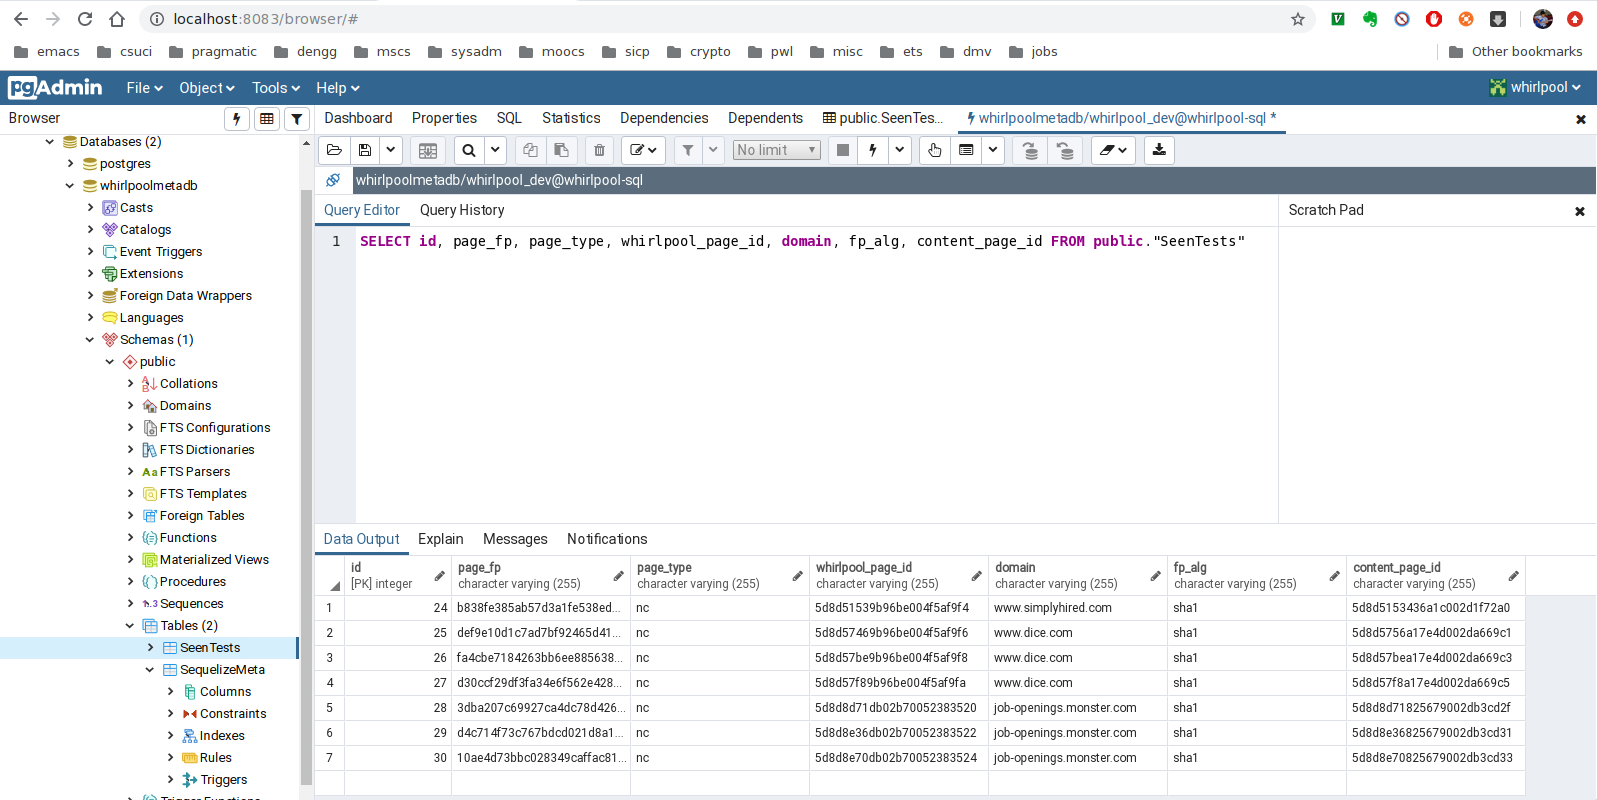
\includegraphics[width=18cm,height=8cm,keepaspectratio]{../media/crawler/fingerprinting.png}
  \caption{document fingerprinting only avoids exact duplicates}
  \label{fig:fingerprinting}
\end{figure}

\noindent
The figure \ref{fig:simhashing} shows entities using \texttt{simhash}\cite{dedupe} function which
internally shingles the words in the document and outputs a single integer(attribute \textttt{page\_fp}).
\begin{figure}[h!]
  \centering
  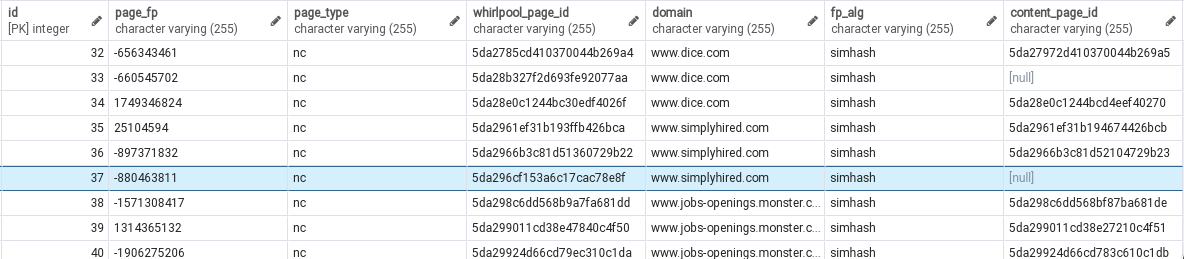
\includegraphics[width=18cm,height=8cm,keepaspectratio]{../media/crawler/shingles.png}
  \caption{near-duplicate detection using shingling\cite{dedupe}}
  \label{fig:simhashing}
\end{figure}

\noindent
A simhash integer of incoming new document is compared against all the available simhashes in the table.
A threshold constant $T$ of less than equal to 0.70 is set during pairwise comparison. 
Any document exceeding $T$ is dropped from mongodb collections except its metadata is saved to postgresDB.
Shingling combined with hashing saves disk space per document and thats exactly why simhash exist.

\pagebreak

\noindent
A bruteforce implementation of pairwise comparison of simhashes has a run time complexity of $O(n^2)$.
Having a dense index such as primary key on attribute \texttt{id} or \texttt{page\_fp} along with
spare index also known as secondary index on attribute \texttt{domain} can speed lookup and decrease disk seeks. The dense index is aware of byte location pointing to blocks, trackers and sectors, whereas, the secondary index inturn points to primary index. This solution only goes so far. A more sustainable improvement
is proposed in next chapter.

\begin{figure}[h!]
  \centering
  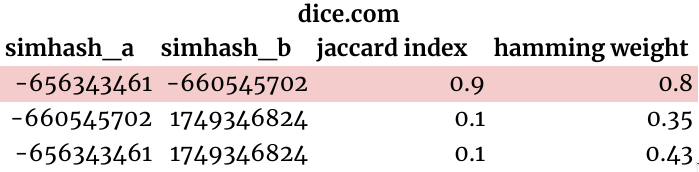
\includegraphics[width=8cm,height=4cm,keepaspectratio]{../media/crawler/dice.png}
  \label{fig:dice}
\end{figure}

\begin{figure}[h!]
  \centering
  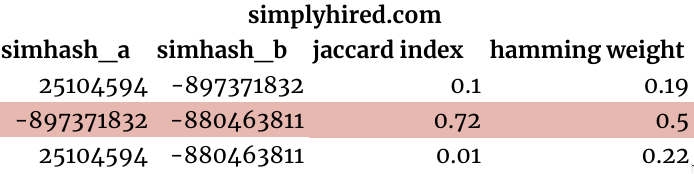
\includegraphics[width=8cm,height=4cm,keepaspectratio]{../media/crawler/simplyhired.png}
  \label{fig:simhired}
\end{figure}

\begin{figure}[h!]
  \centering
  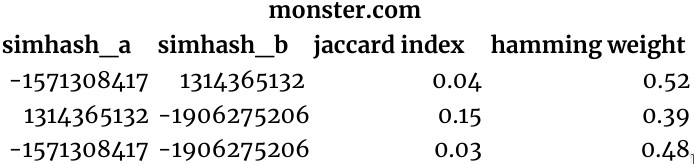
\includegraphics[width=8cm,height=4cm,keepaspectratio]{../media/crawler/monster.png}
  \label{fig:simhired}
\end{figure}

\noindent
Here are few rows of integer hashes belonging to documents crawled. It is showing the similarity between
documents compared. The hashes highlighed in red get dropped for $\geq T$. Similarity is calculated using hamming distance for simhashes and Jaccard Index.
%
%
%\begin{figure}[h!]
%  \centering
%  \includegraphics[width=8cm,height=4cm,keepaspectratio]{../media/crawler/monster.com.png}
%  \label{fig:monster}
%\end{figure}

\pagebreak

\subsection{URL Frontier}
\subsubsection{Prioritizer Policy}
\subsubsection{Front Queue Biased Selection Policy}

\pagebreak